\chapter{统计热力学的应用}\label{ch:b3:statistical-thermo-applied}

储存在最好绝热罐中的液氢仍在蒸发，而且液化后的最初几天里，
蒸发速度远快于经罐壁漏入的热量所能解释的程度。
这部分热量来自液体内部。氢分子以两种形式存在，
两者的差别仅在于其两个质子自旋的相对取向，
且两者之间的转化极其缓慢；
在 \qty{20}{K} 下，一种形式转化为另一种形式所释放的热量，
超过使液体蒸发所需的热量。本章将
在\cref{ch:b3:partition-functions}中建立的配分函数用于热容、
这些核自旋异构体，以及某些晶体在 0 K 时保留的熵，
随后计算平衡常数和同位素效应，
仅需光谱数据。

\begin{recall}
在\Cref{ch:b3:partition-functions}中建立了分子配分函数及其
四个因子，并由此导出 $U$、$S$ 和 $G$。本科二年级分册
建立了标准平衡常数与反应的标准吉布斯自由能之间的关系，
$\Delta_rG^\circ = -RT\ln K^\circ$，并建立了范托夫方程；
在\cref{ch:b3:many-electron-atoms}中指出，交换两个
全同费米子时波函数改变符号；在\cref{ch:b3:rovibrational-spectroscopy}中发现，
\ce{H2} 类分子的转动拉曼光谱中谱线强度呈 3:1 交替。
第一册九年级部分定义了同位素。
\end{recall}

\begin{omfigure}
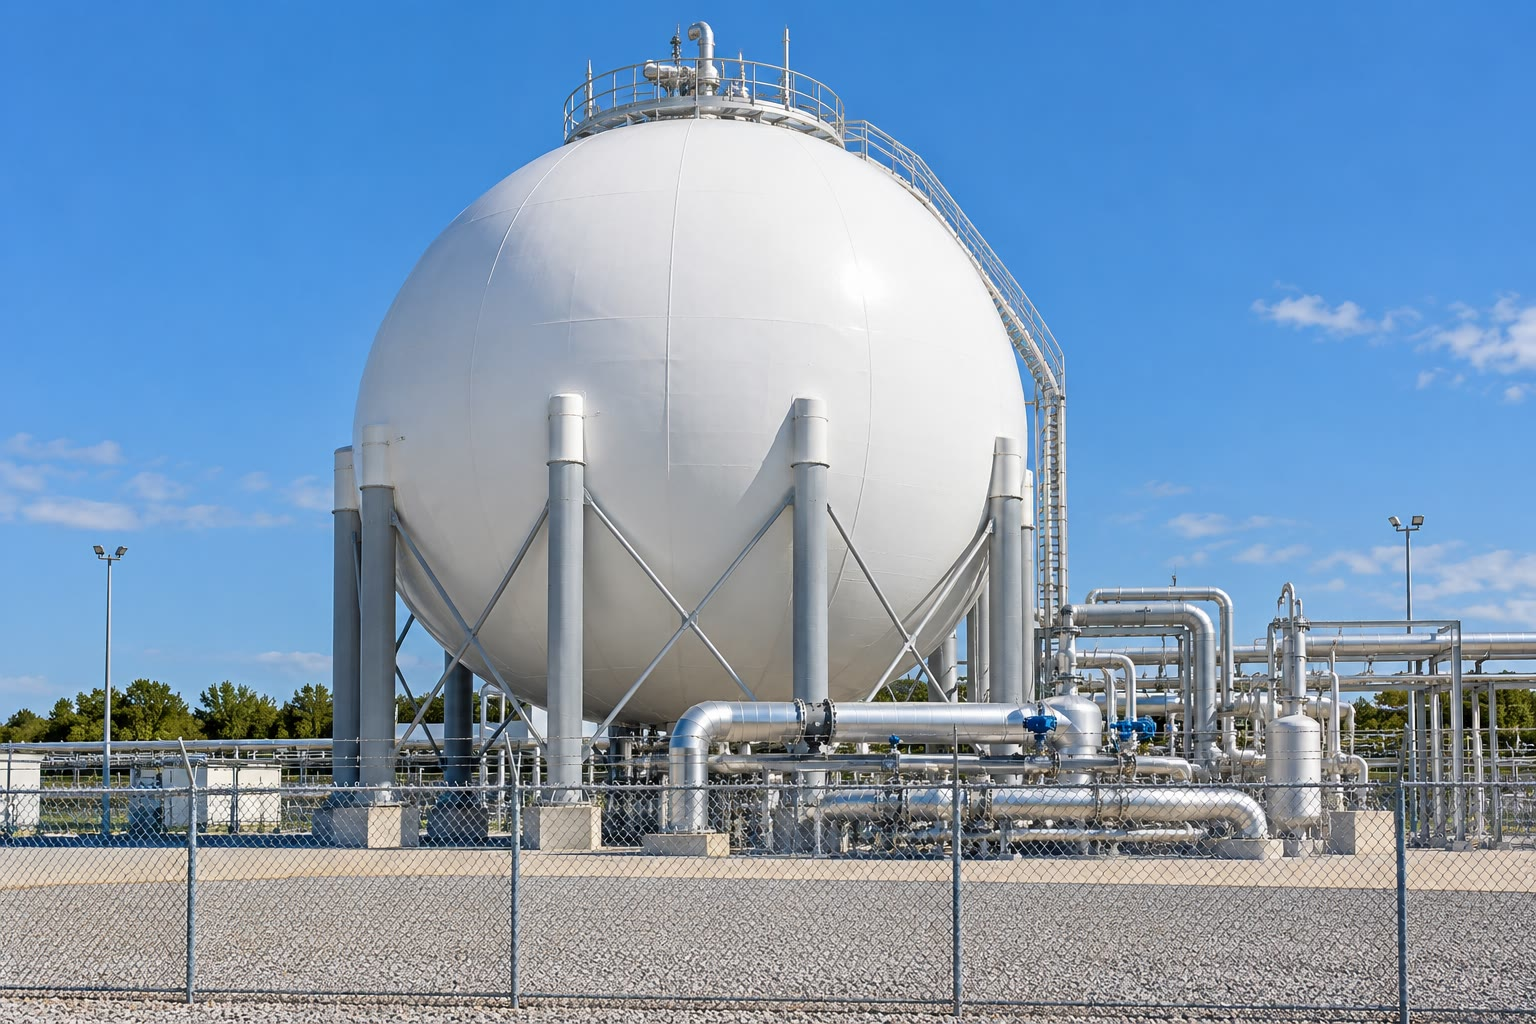
\includegraphics[width=0.6\linewidth]{images/book4/ai/b3-11-lh2-tank.jpg}

{\small 用于液氢的球形储罐。在 \qty{20}{K} 下，液体内部
由氢的一种核自旋形式缓慢转化为另一种而产生的热量，
可以超过从外部漏入的热量。}
\end{omfigure}

\section{气体的热容}

恒容热容为 $C_V = (\partial U/\partial T)_V$，由
\cref{thm:b3:partition-functions:internal-energy}可知，每一类运动
各自独立地作出贡献。两种极限情形决定了全部结论。

\begin{theorem}[能量均分定理]\label{thm:b3:statistical-thermo-applied:equipartition}
当某一运动的能级相对于 $kT$ 十分密集时，
其能量中每个关于坐标或动量的二次项，
对每个分子的平均能量贡献 $\frac12kT$，从而对摩尔
热容贡献 $\frac12R$。此结论称为\emph{能量均分定理}\index{能量均分定理}。
\end{theorem}

\begin{proof}[部分证明]
在经典极限下，某一运动的态求和变为
积分，二次项 $a u^2$ 贡献因子 $\int\eu^{-\beta au^2}\dd u =
\sqrt{\pi/\beta a}$，正比于 $\beta^{-1/2}$。由
\cref{thm:b3:partition-functions:internal-energy}，其平均能量为
$-\partial\ln(\beta^{-1/2})/\partial\beta = 1/2\beta = \frac12kT$。经典积分作为量子求和
的极限，对平动和转动已在
\cref{ch:b3:partition-functions}中证明；对振动则由下一命题
在 $T \gg \theta_{\mathrm V}$ 时得出。
\end{proof}

平动有三个二次项（$\frac32R$）；线性分子转动
有两个（$R$），非线性分子的转动有三个（$\frac32R$）；每个振动有
两个，即动能项与势能项（$R$）。因此，含 $N$ 个原子的线性分子在高温下趋于
$C_{V,\mathrm m} = \frac52R + (3N - 5)R$。该极限在
室温下对振动几乎从未达到。

\begin{proposition}[振动热容]\label{prop:b3:statistical-thermo-applied:cv-vib}
特征温度为 $\theta_{\mathrm V}$ 的简谐振动，其热容贡献为
$x = \theta_{\mathrm V}/T$,
\[
  \frac{C_{V,\mathrm m}^{\mathrm V}}{R} = \frac{x^2\eu^x}{(\eu^x - 1)^2},
\]
上式所示的爱因斯坦函数，当 $T \gg \theta_{\mathrm V}$ 时趋于 1，
并按 $x^2\eu^{-x}$ 指数衰减，对应 $T \ll \theta_{\mathrm V}$ 的情形。
\end{proposition}

\begin{proof}
由\cref{prop:b3:partition-functions:q-vib}可知，每摩尔的 $U - U(0) = R\theta_{\mathrm V}/(\eu^x - 1)$。
对 $T$ 求导，并利用 $\dd x/\dd T = -x/T$，得
$R\theta_{\mathrm V}\eu^x(x/T)/(\eu^x - 1)^2 = Rx^2\eu^x/(\eu^x - 1)^2$。当 $x \to 0$ 时，$\eu^x - 1 \approx x$，该
比值趋于 1；当 $x$ 很大时，它的行为为 $x^2\eu^{-x}$。
\end{proof}

\begin{method}[由简正模式求气体的热容]\label{met:b3:statistical-thermo-applied:cv}
\begin{enumerate}
  \item 平动：$\frac32R$，始终如此。
  \item 转动：线性分子取 $R$，非线性分子取 $\frac32R$，若 $T \gg \theta_{\mathrm R}$，
        对除氢外的所有气体，在几十开尔文以上即成立。
  \item 振动：每个简正模式计入一项爱因斯坦项，其中 $\theta_{\mathrm V} = hc\tilde\nu/k$ 由
        基频波数求得；简并模式计入的次数与其
        简并度相同。
  \item 将各项相加，对理想气体有 $C_{p,\mathrm m} = C_{V,\mathrm m} + R$。
\end{enumerate}
\end{method}

当 $kT$ 相对于某运动的第一激发能很小时，称该运动被冻结：
此时它不携带能量，对 $C_V$ 没有贡献。
\ce{N2} 的振动（$\theta_{\mathrm V} = \qty{3352}{K}$）在室温下被冻结，于是
$C_{V,\mathrm m} = \frac52R$；\ce{Cl2} 的振动（$\theta_{\mathrm V} = \qty{798}{K}$）处于
半激发状态，在 \qty{300}{K} 时 $C_{V,\mathrm m} = 3.07R$。

\begin{omfigure}
\begin{tikzpicture}
\begin{axis}[width=0.86\linewidth, height=6.4cm, xmode=log, xmin=10, xmax=3000,
  ymin=1.3, ymax=3.9, axis lines=left, xlabel={温度 $T$ / K}, ylabel={$C_{V,\mathrm m}/R$},
  tick label style={font=\small}, label style={font=\small},
  log ticks with fixed point, xtick={10,30,100,300,1000,3000},
  unbounded coords=jump]
\addplot[omDef, thick] table[x=T, y=N2] {figdata/out/bachelor-3-heat-capacity.dat};
\addplot[black!60, thick] table[x=T, y=Cl2] {figdata/out/bachelor-3-heat-capacity.dat};
\addplot[omThm, thick, dashed] table[x=T, y=nH2] {figdata/out/bachelor-3-heat-capacity.dat};
\addplot[omThm, thick] table[x=T, y=eH2] {figdata/out/bachelor-3-heat-capacity.dat};
\addplot[only marks, mark=*, mark size=1.6pt, omDef] table[x=T, y=N2] {figdata/out/bachelor-3-heat-capacity-janaf.dat};
\addplot[only marks, mark=square*, mark size=1.5pt, black!60] table[x=T, y=Cl2] {figdata/out/bachelor-3-heat-capacity-janaf.dat};
\draw[black!30, densely dotted] (axis cs:10,1.5) -- (axis cs:3000,1.5);
\draw[black!30, densely dotted] (axis cs:10,2.5) -- (axis cs:3000,2.5);
\draw[black!30, densely dotted] (axis cs:10,3.5) -- (axis cs:3000,3.5);
\node[font=\scriptsize, black!60, anchor=south east] at (axis cs:2900,1.5) {$\frac32$: 平动};
\node[font=\scriptsize, black!60, anchor=south west] at (axis cs:10.5,2.5) {$\frac52$: + 转动};
\node[font=\scriptsize, black!60, anchor=south west] at (axis cs:10.5,3.5) {$\frac72$: + 振动};
\node[font=\scriptsize, omThm, anchor=south west] at (axis cs:60,3.6) {平衡 \ce{H2}};
\node[font=\scriptsize, omThm, anchor=north west] at (axis cs:130,1.78) {常氢 \ce{H2}};
\node[font=\scriptsize, black!70, anchor=south east] at (axis cs:560,3.33) {\ce{Cl2}};
\node[font=\scriptsize, omDef, anchor=south east] at (axis cs:1000,3.0) {\ce{N2}};
\end{axis}
\end{tikzpicture}

{\small 定容摩尔热容，由光谱
常数（谱线；刚性转子、简谐振动）算得，并与热化学表中
\ce{N2} 和 \ce{Cl2} 的数值（点，$C_p/R - 1$）相比较。振动在
$\theta_{\mathrm V}/10$ 附近开始激发；温度高于约 \qty{1000}{K} 时，表中数值高于简谐模型，
简谐模型忽略了非简谐性。氢气的转动贡献，
常氢（虚线，正氢与仲氢按 3:1 冻结）和平衡氢
（实线）。后者超过 $\frac52$，因为仲氢转化为正氢
要吸收热量。}
\end{omfigure}

\section{核自旋统计}

\ce{H2} 的两个原子核是全同费米子，交换它们会使
总波函数变号（见\cref{ch:b3:many-electron-atoms}）。交换二者
等价于使分子端对端翻转，这使转动
波函数 $Y_{J,M}$ 乘以 $(-1)^J$，核自旋函数乘以 $+1$ 或 $-1$。

\begin{theorem}[核自旋统计]\label{thm:b3:statistical-thermo-applied:spin-statistics}
在核自旋为 $I$ 的同核双原子分子中，若其处于基
电子态 ${}^1\Sigma_g^+$，则对称核自旋态有 $(2I+1)(I+1)$ 个，
反对称核自旋态有 $(2I+1)I$ 个。对费米子（$I$ 为半整数），反对称
的与偶数 $J$ 配对，对称的与奇数 $J$ 配对；对玻色子（$I$ 为整数），
情况相反。对 \ce{H2}（$I = \frac12$），偶数与奇数能级的自旋权重分别为
1 和 3；对 \ce{D2}（$I = 1$）为 6 和 3。当 $I = 0$ 时，
只存在一种奇偶性的 $J$：线性 \ce{CO2} 分子，含两个 \ce{^{16}O} 核，且基态对称，
只有偶数转动能级。
\end{theorem}

\begin{proof}[部分证明]
对称性公设（总波函数在两个全同费米子交换下反对称，
玻色子则对称）在本阶段不加证明地承认。单核自旋态的
$(2I+1)^2$ 个乘积 $|m_1\rangle|m_2\rangle$ 给出 $2I+1$ 个对称态
（$m_1 = m_2$），对 $(2I+1)2I/2$ 个满足 $m_1 \ne m_2$ 的配对各有
一个对称组合和一个反对称组合：$(2I+1) + (2I+1)I = (2I+1)(I+1)$
个对称态，$(2I+1)I$ 个反对称态。在 ${}^1\Sigma_g^+$ 态中，电子
与振动函数在交换下不变，因此转动函数与自旋函数的乘积
必须具有所需的总符号。对费米子，
$(-1)^J \times(\text{自旋对称性}) = -1$，此式使偶数 $J$ 与
反对称自旋态配对。对 \ce{H2}：3 个对称态、1 个反对称态；对 \ce{D2}：
6 个与 3 个。
\end{proof}

\begin{definition}[正氢与仲氢]\label{def:b3:statistical-thermo-applied:spin-isomers}
\emph{正氢}\index{正氢}是两个质子自旋处于对称（三重态）
的 \ce{H2} 形式，只占据奇数
转动能级；\emph{仲氢}\index{仲氢}是
自旋态反对称（单重态）的形式，只占据偶数能级。
\end{definition}

两者相互转化需要使一个核自旋相对另一个翻转，
这种翻转与其他氢分子碰撞时几乎不会发生：纯氢中，
两种形式在数天内表现为两种不同的气体。一个顺磁性
表面，其非均匀磁场对两个质子的作用不同，
从而催化这一转化。

\begin{proposition}[平衡正仲氢比]\label{prop:b3:statistical-thermo-applied:ortho-para}
平衡时，仲氢的占比为
\[
  x_{\mathrm{para}} = \frac{\sum_{J\,\mathrm{even}}(2J+1)\eu^{-\theta_{\mathrm R}J(J+1)/T}}
    {\sum_{J\,\mathrm{even}}(2J+1)\eu^{-\theta_{\mathrm R}J(J+1)/T} + 3\sum_{J\,\mathrm{odd}}(2J+1)\eu^{-\theta_{\mathrm R}J(J+1)/T}},
\]
该式在 0 K 时趋于 1，高温时趋于 $\frac14$。对 \ce{D2}，正氢形式
（偶数 $J$）在 0 K 时趋于 1，高温时趋于 $\frac23$。
\end{proposition}

\begin{proof}
取所有态上的玻尔兹曼分布，自旋权重取自
\cref{thm:b3:statistical-thermo-applied:spin-statistics}。0 K 时只有 $J = 0$ 被占据，
它是偶数。高温时，偶数与奇数两项之和各约为
$T/\theta_{\mathrm R}$ 的一半，比值为 $1 : 3$；对 \ce{D2}，为 $6 : 3$。
\end{proof}

对 \ce{H2}，$\theta_{\mathrm R} = \qty{85.4}{K}$：平衡混合物在 \qty{78}{K} 时约半数为仲氢，
在沸点 \qty{20.37}{K} 时仲氢占 99.8\,\%，在室温
下占 25.07\,\%。室温下保存的氢气称为常氢，
因此是正氢与仲氢比为 3:1 的混合物。

\begin{omfigure}
\begin{tikzpicture}
\begin{axis}[width=0.72\linewidth, height=5.4cm, xmin=0, xmax=300, ymin=0, ymax=1.05,
  axis lines=left, xlabel={$T$ / K}, ylabel={平衡分数},
  tick label style={font=\small}, label style={font=\small}]
\addplot[omThm, thick] table[x=T, y=pH2] {figdata/out/bachelor-3-ortho-para.dat};
\addplot[omDef, thick] table[x=T, y=oD2] {figdata/out/bachelor-3-ortho-para.dat};
\draw[black!35, densely dotted] (axis cs:0,0.25) -- (axis cs:300,0.25);
\draw[black!35, densely dotted] (axis cs:0,0.6667) -- (axis cs:300,0.6667);
\node[font=\scriptsize, omThm, anchor=south west] at (axis cs:190,0.27) {\ce{H2} 仲氢占比 $\to \frac14$};
\node[font=\scriptsize, omDef, anchor=south west] at (axis cs:120,0.69) {\ce{D2} 正氢占比 $\to \frac23$};
\end{axis}
\end{tikzpicture}

{\small 核自旋同分异构体的平衡组成随
温度的变化，由转动能级与自旋权重算得（\ce{H2}：权重 1 与 3；
\ce{D2}：6 与 3）。低温时由占据偶数 $J$ 的形式占优。}
\end{omfigure}

氢的热容体现了这些后果。在常氢中，
正氢分子与仲氢分子是按固定比例混合的两种气体，各有各的
能级梯，分别从 $J = 1$ 与 $J = 0$ 开始，两者的转动各自
独立冻结。平衡氢在加热时还会使仲氢转化为正氢，
该过程吸收能量，形成上图中的峰。最早的测量，
未使用催化剂，测得的曲线与常氢曲线一致，而正是对此曲线的
解释——视为冻结的 3:1 混合物——首次揭示了
这两种形式。

\begin{remark}
\cref{prop:b3:partition-functions:q-rot} 中的对称数现已得到说明。
高温时，每个自旋态可占据的转动能级约为一半，
故 $\sum(\text{自旋权重})(2J+1)\eu^{\dots} \approx (2I+1)^2\,T/2\theta_{\mathrm R}$：
按惯例略去总自旋因子 $(2I+1)^2$，保留 $\sigma = 2$。
\end{remark}

\begin{definition}[残余熵]\label{def:b3:statistical-thermo-applied:residual-entropy}
该晶体的\emph{残余熵}\index{残余熵}是指其分子在 $T \to 0$ 时仍保留的熵，
这是因为其分子被冻结在多种
能量相等或近似相等的排列之一中。
\end{definition}

\begin{proposition}[一氧化碳和冰的残余熵]\label{prop:b3:statistical-thermo-applied:residual}
若一块晶体含 $N$ 个分子，它被冻结在 $W_0$ 种等可能的排列中，则 $S_0 =
k\ln W_0$。固态 \ce{CO} 中每个分子的指向有两种可能，故 $S_{0,\mathrm m} = R\ln2 =
\qty{5.76}{J.K^{-1}.mol^{-1}}$。冰中每个氧原子与两个氢原子成键，
并与另外两个分子形成氢键，其 $W_0 = (3/2)^N$，$S_{0,\mathrm m} = R\ln\frac32 =
\qty{3.37}{J.K^{-1}.mol^{-1}}$。
\end{proposition}

\begin{proof}
在 $T \to 0$ 下应用\cref{def:b3:partition-functions:statistical-entropy}。
对于 \ce{CO}：分子偶极矩极小，使取向 CO 与 OC 的能量几乎相同，
两者能量几乎相等；$N$ 个分子各有两种取向，故 $W_0 = 2^N$，
$S_0 = Nk\ln2$。对于冰（采用鲍林的计数方法），$2N$ 个氢原子各位于一条
O$\cdots$O 连线上，靠近其中一端，共 $2^{2N}$ 种排布。在一个氧原子周围放置四个氢原子的 16 种方式中，
有 6 种使该氧原子恰好有两个近邻氢原子，
即一个水分子；将各氧原子视为相互独立，则
每个氧原子满足该条件的排布比例为 $6/16$，故 $W_0 = 2^{2N}(6/16)^N = (3/2)^N$。
\end{proof}

表中给出的 \ce{CO} 统计熵
（见\cref{ch:b3:partition-functions}）；量热熵比它低的差值约为
$R\ln2$ 量级，因取向并非完全随机，
故该差值略小一些。对于冰，水蒸气的量热熵与其统计熵之差，
其统计值与鲍林于 1935 年提出计数时的结果相符，
由此证实冰中质子是无序的。热力学第三定律
其表述为“完美晶体在 0 K 时的熵为零”，它适用于
能达到唯一排列的晶体。

\begin{omfigure}
\begin{tikzpicture}[scale=1.15, every node/.style={transform shape}]
  \draw[black!45, dashed] (0.00,0.00) -- (1.20,0.00);
  \draw[black, thick] (0.00,0.00) -- (0.36,0.00); \node[aH, minimum size=2.2mm] at (0.36,0.00) {};
  \draw[black!45, dashed] (0.00,0.00) -- (0.00,1.20);
  \draw[black, thick] (0.00,0.00) -- (0.00,0.36); \node[aH, minimum size=2.2mm] at (0.00,0.36) {};
  \draw[black!45, dashed] (0.00,1.20) -- (1.20,1.20);
  \draw[black, thick] (0.00,1.20) -- (0.36,1.20); \node[aH, minimum size=2.2mm] at (0.36,1.20) {};
  \draw[black!45, dashed] (0.00,1.20) -- (0.00,2.40);
  \draw[black, thick] (0.00,2.40) -- (0.00,2.04); \node[aH, minimum size=2.2mm] at (0.00,2.04) {};
  \draw[black!45, dashed] (0.00,2.40) -- (1.20,2.40);
  \draw[black, thick] (1.20,2.40) -- (0.84,2.40); \node[aH, minimum size=2.2mm] at (0.84,2.40) {};
  \draw[black!45, dashed] (0.00,2.40) -- (0.00,3.60);
  \draw[black, thick] (0.00,3.60) -- (0.00,3.24); \node[aH, minimum size=2.2mm] at (0.00,3.24) {};
  \draw[black!45, dashed] (0.00,3.60) -- (1.20,3.60);
  \draw[black, thick] (1.20,3.60) -- (0.84,3.60); \node[aH, minimum size=2.2mm] at (0.84,3.60) {};
  \draw[black!45, dashed] (0.00,3.60) -- (0.00,4.20);
  \draw[black, thick] (0.00,3.60) -- (0.00,3.96); \node[aH, minimum size=2.2mm] at (0.00,3.96) {};
  \draw[black!45, dashed] (1.20,0.00) -- (2.40,0.00);
  \draw[black, thick] (1.20,0.00) -- (1.56,0.00); \node[aH, minimum size=2.2mm] at (1.56,0.00) {};
  \draw[black!45, dashed] (1.20,0.00) -- (1.20,1.20);
  \draw[black, thick] (1.20,1.20) -- (1.20,0.84); \node[aH, minimum size=2.2mm] at (1.20,0.84) {};
  \draw[black!45, dashed] (1.20,1.20) -- (2.40,1.20);
  \draw[black, thick] (2.40,1.20) -- (2.04,1.20); \node[aH, minimum size=2.2mm] at (2.04,1.20) {};
  \draw[black!45, dashed] (1.20,1.20) -- (1.20,2.40);
  \draw[black, thick] (1.20,1.20) -- (1.20,1.56); \node[aH, minimum size=2.2mm] at (1.20,1.56) {};
  \draw[black!45, dashed] (1.20,2.40) -- (2.40,2.40);
  \draw[black, thick] (1.20,2.40) -- (1.56,2.40); \node[aH, minimum size=2.2mm] at (1.56,2.40) {};
  \draw[black!45, dashed] (1.20,2.40) -- (1.20,3.60);
  \draw[black, thick] (1.20,3.60) -- (1.20,3.24); \node[aH, minimum size=2.2mm] at (1.20,3.24) {};
  \draw[black!45, dashed] (1.20,3.60) -- (2.40,3.60);
  \draw[black, thick] (2.40,3.60) -- (2.04,3.60); \node[aH, minimum size=2.2mm] at (2.04,3.60) {};
  \draw[black!45, dashed] (1.20,3.60) -- (1.20,4.20);
  \draw[black!45, dashed] (2.40,0.00) -- (3.60,0.00);
  \draw[black, thick] (3.60,0.00) -- (3.24,0.00); \node[aH, minimum size=2.2mm] at (3.24,0.00) {};
  \draw[black!45, dashed] (2.40,0.00) -- (2.40,1.20);
  \draw[black, thick] (2.40,0.00) -- (2.40,0.36); \node[aH, minimum size=2.2mm] at (2.40,0.36) {};
  \draw[black!45, dashed] (2.40,1.20) -- (3.60,1.20);
  \draw[black, thick] (2.40,1.20) -- (2.76,1.20); \node[aH, minimum size=2.2mm] at (2.76,1.20) {};
  \draw[black!45, dashed] (2.40,1.20) -- (2.40,2.40);
  \draw[black, thick] (2.40,2.40) -- (2.40,2.04); \node[aH, minimum size=2.2mm] at (2.40,2.04) {};
  \draw[black!45, dashed] (2.40,2.40) -- (3.60,2.40);
  \draw[black, thick] (3.60,2.40) -- (3.24,2.40); \node[aH, minimum size=2.2mm] at (3.24,2.40) {};
  \draw[black!45, dashed] (2.40,2.40) -- (2.40,3.60);
  \draw[black, thick] (2.40,2.40) -- (2.40,2.76); \node[aH, minimum size=2.2mm] at (2.40,2.76) {};
  \draw[black!45, dashed] (2.40,3.60) -- (3.60,3.60);
  \draw[black, thick] (2.40,3.60) -- (2.76,3.60); \node[aH, minimum size=2.2mm] at (2.76,3.60) {};
  \draw[black!45, dashed] (2.40,3.60) -- (2.40,4.20);
  \draw[black!45, dashed] (3.60,0.00) -- (4.20,0.00);
  \draw[black, thick] (3.60,0.00) -- (3.96,0.00); \node[aH, minimum size=2.2mm] at (3.96,0.00) {};
  \draw[black!45, dashed] (3.60,0.00) -- (3.60,1.20);
  \draw[black, thick] (3.60,1.20) -- (3.60,0.84); \node[aH, minimum size=2.2mm] at (3.60,0.84) {};
  \draw[black!45, dashed] (3.60,1.20) -- (4.20,1.20);
  \draw[black!45, dashed] (3.60,1.20) -- (3.60,2.40);
  \draw[black, thick] (3.60,1.20) -- (3.60,1.56); \node[aH, minimum size=2.2mm] at (3.60,1.56) {};
  \draw[black!45, dashed] (3.60,2.40) -- (4.20,2.40);
  \draw[black!45, dashed] (3.60,2.40) -- (3.60,3.60);
  \draw[black, thick] (3.60,2.40) -- (3.60,2.76); \node[aH, minimum size=2.2mm] at (3.60,2.76) {};
  \draw[black!45, dashed] (3.60,3.60) -- (4.20,3.60);
  \draw[black, thick] (3.60,3.60) -- (3.96,3.60); \node[aH, minimum size=2.2mm] at (3.96,3.60) {};
  \draw[black!45, dashed] (3.60,3.60) -- (3.60,4.20);
  \draw[black, thick] (3.60,3.60) -- (3.60,3.96); \node[aH, minimum size=2.2mm] at (3.60,3.96) {};
  \draw[black!45, dashed] (-0.60,0.00) -- (0.00,0.00);
  \draw[black!45, dashed] (-0.60,1.20) -- (0.00,1.20);
  \draw[black, thick] (0.00,1.20) -- (-0.36,1.20); \node[aH, minimum size=2.2mm] at (-0.36,1.20) {};
  \draw[black!45, dashed] (-0.60,2.40) -- (0.00,2.40);
  \draw[black, thick] (0.00,2.40) -- (-0.36,2.40); \node[aH, minimum size=2.2mm] at (-0.36,2.40) {};
  \draw[black!45, dashed] (-0.60,3.60) -- (0.00,3.60);
  \draw[black!45, dashed] (0.00,-0.60) -- (0.00,0.00);
  \draw[black!45, dashed] (1.20,-0.60) -- (1.20,0.00);
  \draw[black, thick] (1.20,0.00) -- (1.20,-0.36); \node[aH, minimum size=2.2mm] at (1.20,-0.36) {};
  \draw[black!45, dashed] (2.40,-0.60) -- (2.40,0.00);
  \draw[black, thick] (2.40,0.00) -- (2.40,-0.36); \node[aH, minimum size=2.2mm] at (2.40,-0.36) {};
  \draw[black!45, dashed] (3.60,-0.60) -- (3.60,0.00);
  \node[aO, minimum size=4mm] at (0.00,0.00) {};
  \node[aO, minimum size=4mm] at (0.00,1.20) {};
  \node[aO, minimum size=4mm] at (0.00,2.40) {};
  \node[aO, minimum size=4mm] at (0.00,3.60) {};
  \node[aO, minimum size=4mm] at (1.20,0.00) {};
  \node[aO, minimum size=4mm] at (1.20,1.20) {};
  \node[aO, minimum size=4mm] at (1.20,2.40) {};
  \node[aO, minimum size=4mm] at (1.20,3.60) {};
  \node[aO, minimum size=4mm] at (2.40,0.00) {};
  \node[aO, minimum size=4mm] at (2.40,1.20) {};
  \node[aO, minimum size=4mm] at (2.40,2.40) {};
  \node[aO, minimum size=4mm] at (2.40,3.60) {};
  \node[aO, minimum size=4mm] at (3.60,0.00) {};
  \node[aO, minimum size=4mm] at (3.60,1.20) {};
  \node[aO, minimum size=4mm] at (3.60,2.40) {};
  \node[aO, minimum size=4mm] at (3.60,3.60) {};
\end{tikzpicture}

{\small 冰中的质子无序，画成平面方格网络（真实
网络为四面体形）：每个氧（红色）有四个 O$\cdots$O 近邻，每条线上
恰有一个氢（白色），且与之靠近的氢恰有两个（冰
规则）。这是鲍林计数中 $(3/2)^N$ 种排列之一；所有排列
的能量几乎相同，冻结时随机选取其中一种。}
\end{omfigure}

\section{由配分函数求平衡常数}

\begin{theorem}[由配分函数求平衡常数]\label{thm:b3:statistical-thermo-applied:k-from-q}
对理想气体间的反应 $0 = \sum_J\nu_J\mathrm J$，
\[
  K^\circ = \prod_J\Bigl(\frac{q^\circ_{J,\mathrm m}}{N_A}\Bigr)^{\nu_J}\eu^{-\Delta_rE_0/RT},
\]
其中 $q^\circ_{J,\mathrm m}$ 为 $\mathrm J$ 在标准摩尔体积
$V^\circ_{\mathrm m} = RT/p^\circ$ 下的配分函数，各自从其自身基态算起，且 $\Delta_rE_0 =
\sum\nu_JE_{0,J}$ 为 0 K 时的反应摩尔能量，即从反应物基态
至生成物的基态。
\end{theorem}

\begin{proof}
由\cref{thm:b3:partition-functions:entropy}可知，一摩尔理想气体 $\mathrm J$ 在 $p^\circ$ 下有
$G^\circ_{\mathrm m} - G_{\mathrm m}(0) = -RT\ln(q^\circ_{J,\mathrm m}/N_A)$，且 $G_{\mathrm m}(0)$ 是
其基态能量 $E_{0,J}$，取所有物种共同的能量标度。于是 $\Delta_rG^\circ =
\Delta_rE_0 - RT\sum_J\nu_J\ln(q^\circ_{J,\mathrm m}/N_A)$，再由 $\Delta_rG^\circ = -RT\ln K^\circ$ 即
得结论。
\end{proof}

\begin{method}[由光谱数据计算平衡常数]\label{met:b3:statistical-thermo-applied:k-stat}
\begin{enumerate}
  \item 对每个物种，$q^\circ_{\mathrm m}/N_A = (kT/p^\circ)\Lambda^{-3}\times q^{\mathrm R}q^{\mathrm V}q^{\mathrm E}$，
        并计入对称数和电子简并度。
  \item $\Delta_rE_0$ 取自离解能 $D_0$（自基态
        振动能级起算，故已包含零点能），或取自
        0 K 时的生成焓。
  \item 相乘，并检查单位：$K^\circ$ 为纯数，
        标准压强经 $kT/p^\circ$ 引入。
\end{enumerate}
\end{method}

\begin{example}[碘的离解]\label{ex:b3:statistical-thermo-applied:iodine}
% ledger: janaf:I.dfH0, janaf:I2g.dfH0, lev:I.2P1_2, diat:I2.we, diat:I2.wexe, diat:I2.Be, diat:I2.ae, aw:I, janaf:I.logKf.1000
对于 $\ce{I2(g) <=> 2 I(g)}$，$\Delta_rE_0 = D_0(\ce{I2}) = 2 \times 107.164 - 65.504 = \qty{148.824}{kJ/mol}$
由热化学数据表中 0 K 时的生成焓得到。在
\qty{1000}{K} 下：对 I，$\Lambda = \qty{4.90}{pm}$，$kT/p^\circ = \qty{1.381e-25}{m^3}$，$q^{\mathrm E} = 4 +
2\eu^{-10.94} = 4.0000$（${}^2P_{1/2}$ 能级高出 \qty{7603}{cm^{-1}}），故 $q^\circ_{\mathrm m}/N_A = \num{4.69e9}$；
对 \ce{I2}，$\Lambda = \qty{3.47}{pm}$，$q^{\mathrm R} = 1000/(2 \times 0.05369) = 9313$，且 $q^{\mathrm V} = 3.784$，故
$q^\circ_{\mathrm m}/N_A = \num{1.17e14}$。于是 $K^\circ = (4.69\times10^9)^2/(1.17\times10^{14}) \times \eu^{-17.90} =
\num{3.17e-3}$，$\log K^\circ = -2.50$；热化学表给出 $-2.51$。
\end{example}

\begin{omfigure}
\begin{tikzpicture}
\begin{axis}[name=ki, width=0.5\linewidth, height=5.6cm, xmin=0.58, xmax=1.45, ymin=-6.5,
  ymax=1, axis lines=left, xlabel={$1000\,\mathrm K/T$}, ylabel={$\log K^\circ$},
  tick label style={font=\small}, label style={font=\small},
  title={\small $\ce{I2 <=> 2 I}$}]
\addplot[black, thick] table[x=invT, y=logK] {figdata/out/bachelor-3-equilibrium-constant-stat-i2.dat};
\addplot[only marks, mark=*, mark size=1.8pt, omThm] table[x=invT, y=logK] {figdata/out/bachelor-3-equilibrium-constant-stat-i2-janaf.dat};
\node[font=\scriptsize, anchor=north east, align=right] at (axis cs:1.43,0.8) {线：统计 \\ 点：热化学表};
\end{axis}
\begin{axis}[at={(ki.east)}, anchor=west, xshift=1.4cm, width=0.44\linewidth, height=5.6cm,
  xmin=0, xmax=2000, ymin=0, ymax=4.4, axis lines=left, xlabel={$T$ / K},
  ylabel={$K^\circ$}, tick label style={font=\small}, label style={font=\small},
  title={\small $\ce{H2 + D2 <=> 2 HD}$}, scaled x ticks=false,
  xticklabel style={/pgf/number format/1000 sep={}}]
\addplot[omDef, thick] table[x=T, y=K] {figdata/out/bachelor-3-equilibrium-constant-stat-hd.dat};
\draw[black!35, densely dotted] (axis cs:0,4) -- (axis cs:2000,4);
\node[font=\scriptsize, anchor=north east] at (axis cs:1950,3.95) {$\sigma$ 极限：4};
\end{axis}
\end{tikzpicture}

{\small 由配分函数算得的平衡常数。左图为碘的
离解，为斜率 $-\Delta_rH^\circ/(R\ln10)$ 的范托夫直线，并
标出热化学表的数值（数据点）。右图为交换反应 $\ce{H2 + D2
<=> 2 HD}$，其在高温时趋于对称数之比 4，
而在低温时则经零点能与
核自旋的限制而低于此值。}
\end{omfigure}

\begin{proposition}[H$_2$ + D$_2$ 交换反应]\label{prop:b3:statistical-thermo-applied:hd}
对于 $\ce{H2 + D2 <=> 2 HD}$，高温时 $K^\circ \to 4$。
\end{proposition}

\begin{proof}
高温时，平动、转动和振动因子分别为
$m^{3/2}$，$T/\sigma\theta_{\mathrm R} \propto \mu/\sigma$ 和 $T/\theta_{\mathrm V} \propto \sqrt\mu$（力常数是一个
电子性质，对三种分子相同），且 $\Delta_rE_0/RT \to 0$。
取 $m_{\ce{H2}} = 2$，$m_{\ce{D2}} = 4$，$m_{\ce{HD}} = 3$，且 $\mu = 1/2$、1、$2/3$（以
质子质量为单位，忽略 D 与 2H 之间的微小差别）：
\[
  K^\circ \to \Bigl(\frac{9}{8}\Bigr)^{3/2} \times \frac{(2/3)^2/1^2}{(1/2)(1)/(2 \times 2)}
  \times \frac{2/3}{\sqrt{1/2}\sqrt1}
  = \frac{27}{16\sqrt2} \times \frac{32}{9} \times \frac{2\sqrt2}{3} = 4 .
\]
质量因子全部精确相消，只剩对称数，$\sigma_{\ce{H2}}
\sigma_{\ce{D2}}/\sigma_{\ce{HD}}^2 = 4$。
\end{proof}

在 \qty{298.15}{K} 时统计常数为 3.26：\ce{H2}、
\ce{D2} 与 HD 的零点能（\qty{2170.3}{cm^{-1}}、\qty{1542.3}{cm^{-1}} 与 \qty{1883.7}{cm^{-1}}）给出 $\Delta_rE_0 =
\qty{54.8}{cm^{-1}}$，因子为 $\eu^{-54.8/207.2} = 0.77$；转动仍部分量子化，
对这些轻分子亦不可忽略。

\begin{proposition}[范托夫方程的再推导]\label{prop:b3:statistical-thermo-applied:vant-hoff-stat}
统计平衡常数满足 $\dfrac{\dd\ln K^\circ}{\dd T} = \dfrac{\Delta_rH^\circ}{RT^2}$。
\end{proposition}

\begin{proof}
每个 $q^\circ_{J,\mathrm m}$ 依赖于 $T$，既通过其能级，也通过 $V^\circ_{\mathrm m} = RT/p^\circ$：
$\dd\ln q^\circ_{J,\mathrm m}/\dd T = (U_J - U_J(0))/RT^2 + 1/T$，按每摩尔计，由
\cref{thm:b3:partition-functions:internal-energy}可知。于是 $\dd\ln K^\circ/\dd T =
[\Delta_rE_0 + \sum\nu_J(U_J - U_J(0)) + \sum\nu_JRT]/RT^2 = (\Delta_rU + \Delta\nu_{\mathrm g}RT)/RT^2 =
\Delta_rH^\circ/RT^2$，对理想气体成立。
\end{proof}

由图左侧面板的斜率可得，碘在 \qty{1000}{K} 附近的解离焓为
\qty{154}{kJ/mol}：即 $D_0$ 加上两个原子相对于一个分子多出的平动
能，再减去分子的转动
能与振动能。

\section{同位素效应}

同位素异构体的电子结构相同，因而具有相同的
势能曲线和力常数，但质量不同，其振动波数、零点能
和配分函数各不相同，
平衡常数也随之不同。

\begin{definition}[平衡同位素效应、分馏系数、$\delta$ 值]\label{def:b3:statistical-thermo-applied:isotope-effect}
某反应的\emph{平衡同位素效应}\index{平衡同位素效应}为其在轻、重同位素下平衡常数之比，
即 $K_{\mathrm{light}}/K_{\mathrm{heavy}}$。
两相或两种化合物 A 与 B 之间的\emph{分馏系数}\index{分馏系数}为
$\alpha_{\mathrm{A/B}} = R_{\mathrm A}/R_{\mathrm B}$，其中 $R$ 为重同位素与轻同位素之比
（例如 $\ce{^{18}O}/\ce{^{16}O}$）。
某样品的\emph{$\delta$ 值}\index{$\delta$ 值}为 $\delta = (R_{\mathrm{sample}}/R_{\mathrm{standard}}
- 1) \times 1000$，以千分率（\textperthousand）表示。
\end{definition}

\begin{proposition}[由零点能导出的同位素效应]\label{prop:b3:statistical-thermo-applied:zpe-isotope}
对交换反应 $\ce{XH + YD <=> XD + YH}$，在伸缩振动冻结的温度下，
平衡常数的主导因子为
\[
  K \approx \exp\Bigl(-\frac{\Delta\mathrm{ZPE}}{kT}\Bigr), \qquad
  \Delta\mathrm{ZPE} = \tfrac12hc\bigl[\tilde\nu_{\mathrm{XD}} + \tilde\nu_{\mathrm{YH}} - \tilde\nu_{\mathrm{XH}} - \tilde\nu_{\mathrm{YD}}\bigr],
\]
对与重原子相连的氢，$\tilde\nu_{\mathrm D} \approx \tilde\nu_{\mathrm H}/\sqrt2$。重
同位素富集于较硬的键中。
\end{proposition}

\begin{proof}
由 \Cref{thm:b3:statistical-thermo-applied:k-from-q} 可得，能量自共同势能曲线
的底部起算，$\Delta_rE_0$ 即零点能的变化。
平动因子与转动因子近似相消，
这在重伴侣上同种同位素的两次交换之间成立，并且
冻结时振动配分函数为 1。由 $\tilde\nu \propto \mu^{-1/2}$ 及
对重原子 X 有 $\mu_{\mathrm{XD}} \approx 2\mu_{\mathrm{XH}}$，$\tilde\nu_{\mathrm{XD}} = \tilde\nu_{\mathrm{XH}}/\sqrt2$，于是 $\Delta\mathrm{ZPE} =
\frac12hc(1 - 1/\sqrt2)(\tilde\nu_{\mathrm{YH}} - \tilde\nu_{\mathrm{XH}})$，其值为负，故 $K > 1$，当 X--H 为
较硬的键时如此。
\end{proof}

同样的推理也可解释氧同位素在水与其蒸气之间、
水与贝壳碳酸盐之间以及两种矿物之间的分馏。
分馏系数在高温下趋于 1（正如 $K_{\mathrm{HD}}$
趋于其对称极限那样），随温度降低而偏离 1。
以 $\delta$ 值表示时，它是一种温度计：化石贝壳碳酸盐的 $\delta^{18}$O
记录了其生长时水体的温度，而
极地冰芯中冰的记录
则反映了形成其雪层的云的温度。

\begin{inthelab}[正–仲氢转换器]
氢液化器分级冷却气体，并在各级之间使其通过
顺磁性催化剂床层，通常为水合氧化铁(III)。
每一温度下，转化热由制冷机移走，
到达储罐的液体接近其平衡组成，
几乎全部为仲氢。若无催化剂，转化热
将在储罐中释放。
\end{inthelab}

\begin{safety}{\ghs[0.8cm]{GHS02}\ghs[0.8cm]{GHS04}}
% ledger: ghs:H2
氢：一种极易燃的气体，以加压或低温液体形式储存，
与空气在很宽的范围内形成爆炸性混合物，燃烧时火焰几乎不可见；
液体会造成冻伤，其蒸气会
排挤空气。
\end{safety}

\begin{history}[两种氢，1927--1929]
1927 年，海森堡与洪特预言，氢分子应以两种形式存在，
二者因核自旋不同而有所区别；同年，丹尼森证明，室温以下测得的
氢的反常热容，正是两者按 3:1 混合、
冻结于室温组成时的热容。1929 年，邦霍弗与哈特克将氢吸附于
活性炭上，在液态空气温度下脱附得到
几乎纯的仲氢，依其热导率不同而加以辨认，
并发现它只非常缓慢地
转回正常混合物。
\end{history}

\section{练习}

\begin{exercise}[$\star$]\label{exo:b3:statistical-thermo-applied:1}
求 \ce{CO2}（直线形，3 个原子）的 $C_{V,\mathrm m}$ 的高温极限，并说明
室温下哪些贡献仍被冻结。
\end{exercise}

\begin{exercise}[$\star$]\label{exo:b3:statistical-thermo-applied:2}
计算爱因斯坦函数在 $T = \theta_{\mathrm V}$ 与 $T = \theta_{\mathrm V}/10$ 处的值。
\end{exercise}

\begin{exercise}[$\star$]\label{exo:b3:statistical-thermo-applied:3}
% ledger: diat:H2.Be, diat:H2.ae
已知 \ce{H2} 的 $\theta_{\mathrm R} = \qty{85.35}{K}$，计算
在 \qty{20}{K} 时（只需 $J = 0$ 与 $J = 1$）以及在 \qty{77}{K} 时（$J \le 3$）的平衡仲氢分数。
\end{exercise}

\begin{exercise}[$\star$]\label{exo:b3:statistical-thermo-applied:4}
解释为什么氘（核自旋为 1）的正、仲权重比为 $6 : 3$，
以及在 0 K 时哪种形式稳定，并求室温下的比值。
\end{exercise}

\begin{exercise}[$\star\star$]\label{exo:b3:statistical-thermo-applied:5}
% ledger: diat:H2.we, diat:H2.wexe, diat:D2.we, diat:D2.wexe, diat:HD.we, diat:HD.wexe
\ce{H2}、\ce{D2} 和 HD 的零点能分别为 2170.3、1542.3 和
\qty{1883.7}{cm^{-1}}。计算 $\Delta_rE_0$（对于反应 $\ce{H2 + D2 <=> 2 HD}$）以及
因子 $\eu^{-\Delta_rE_0/RT}$ 在 \qty{298.15}{K} 时的值，并将 $4\eu^{-\Delta_rE_0/RT}$ 与完整统计值 3.26 进行比较。
\end{exercise}

\begin{exercise}[$\star\star$]\label{exo:b3:statistical-thermo-applied:6}
估算 \ce{N2O} 晶体的残余熵（线性 NNO，可以
任一方向取向），以及 \ce{CH3D} 晶体的残余熵（其 D 可以占据四个
位置中的任意一个）。
\end{exercise}

\begin{exercise}[$\star\star$]\label{exo:b3:statistical-thermo-applied:7}
% ledger: diat:Cl2.we, diat:Cl2.wexe, janaf:Cl2.Cp.300
计算 \ce{Cl2} 在 \qty{300}{K} 时的 $C_{p,\mathrm m}$，由 $\theta_{\mathrm V} = \qty{797.6}{K}$ 出发，并与
表列的 \qty{33.981}{J.K^{-1}.mol^{-1}} 比较。
\end{exercise}

\begin{exercise}[$\star\star$]\label{exo:b3:statistical-thermo-applied:8}
% ledger: diat:I2.we, diat:I2.wexe
计算 \ce{I2} 的振动热容（$\theta_{\mathrm V} = \qty{306.9}{K}$）在
\qty{298.15}{K} 时的值，以其能量均分值的分数表示。
\end{exercise}

\begin{exercise}[$\star\star$]\label{exo:b3:statistical-thermo-applied:9}
水样 A 的 $\delta^{18}\mathrm O = -10.0$\,\textperthousand，水样 B 的
$+2.0$\,\textperthousand（同一标度）。哪一个更富集 \ce{^{18}O}？计算
分馏系数 $\alpha_{\mathrm{A/B}}$。
\end{exercise}

\begin{exercise}[$\star\star\star$]\label{exo:b3:statistical-thermo-applied:10}
在交换反应 $\ce{XH + YD <=> XD + YH}$（数据同本练习）中，$\tilde\nu_{\mathrm{XH}} =
\qty{3000}{cm^{-1}}$，$\tilde\nu_{\mathrm{YH}} = \qty{2000}{cm^{-1}}$，X 和 Y 为重原子。估算 $K$ 在
\qty{298.15}{K} 时的值，并说明氘原子去向何处。
\end{exercise}

\begin{exercise}[$\star\star\star$]\label{exo:b3:statistical-thermo-applied:11}
% ledger: janaf:I.dfH0, janaf:I2g.dfH0, lev:I.2P1_2, diat:I2.we, diat:I2.wexe, diat:I2.Be, diat:I2.ae, aw:I
$\ce{I2 <=> 2 I}$ 的统计常数为：在 \qty{900}{K} 时 $\log K^\circ = -3.392$，且
在 \qty{1100}{K} 时为 $-1.766$。求区间内的平均 $\Delta_rH^\circ$，并
解释其为什么大于 $D_0 = \qty{148.8}{kJ/mol}$。
\end{exercise}

\begin{exercise}[$\star\star\star$]\label{exo:b3:statistical-thermo-applied:12}
对低温下的仲氢，只有 $J = 0$ 和 $J = 2$ 起作用。证明
其转动热容为 $C/R = 5x^2\eu^{-x}/(1 + 5\eu^{-x})^2$，其中 $x = 6\theta_{\mathrm R}/T$，并
求其在 \qty{100}{K} 时的值（$\theta_{\mathrm R} = \qty{85.35}{K}$）。
\end{exercise}

\section{问题：储存液氢}

\begin{problem}[{周末问题——储存液氢：两种
核自旋形态、它们转化时的热、由此引起的蒸发损失，
以及阻止这一损失的催化剂}]
\label{pb:b3:statistical-thermo-applied:1}
% ledger: diat:H2.Be, diat:H2.ae, diat:H2.De, hvap:nH2, tb:nH2, aw:H
氢在 \qty{1.01325}{bar} 压强下于沸点 \qty{20.37}{K} 液化，此时其
汽化焓为 \qty{0.905}{kJ/mol}。转动能级为 $F(J) = B_0J(J+1) -
D J^2(J+1)^2$，其中 $B_0 = \qty{59.322}{cm^{-1}}$，$D = \qty{0.0471}{cm^{-1}}$（$\theta_{\mathrm R} = \qty{85.35}{K}$）。
摩尔质量为 \qty{2.016}{g/mol}。液态中未催化的正氢 $\to$ 仲氢转化
取为一级反应，$k = \qty{0.0114}{h^{-1}}$（本题数据）。

\medskip\noindent\textbf{第一部分——两种形态。}
\begin{enumerate}
  \item 一对质子有多少种核自旋态？其中有几个对交换对称、
        几个对交换反对称？
  \item 哪些自旋态对应偶数 $J$，哪些对应奇数 $J$？为什么？
  \item 给出偶数能级与奇数能级的自旋权重。
  \item 证明室温下氢的正、仲比为 3:1。
  \item 计算 $J = 1$ 能级高于 $J = 0$ 的能量，分别以 \unit{cm^{-1}} 和
        \unit{kJ/mol} 表示。
  \item 计算 \qty{20.37}{K} 时平衡态的仲氢分数。
  \item 平衡混合物在约 \qty{78}{K} 时仲氢占一半。为什么该温度
        接近 $\theta_{\mathrm R}$？
\end{enumerate}

\medskip\noindent\textbf{第二部分——转化热。}
\begin{enumerate}[resume]
  \item 刚液化的氢在不加催化剂时，其正氢的
        分数是多少？为什么液化过程中它不会改变？
  \item 计算一摩尔该氢在
        \qty{20.37}{K} 下达到平衡时放出的热。
  \item 以每千克表示该热量。
  \item 以每千克表示汽化焓。
  \item 比较二者。
  \item 为什么改进储罐的绝热也无法消除这部分热？
\end{enumerate}

\medskip\noindent\textbf{第三部分——蒸发损失。}
\begin{enumerate}[resume]
  \item 给出储罐中经过时间 $t$ 后的正氢分数。
  \item 计算经过 \qty{24}{h} 后的值。
  \item 计算前 \qty{24}{h} 内每摩尔液体放出的热。
  \item 这些热量能使多大比例的液体蒸发？
  \item 对一周重复上述计算。为什么这种简单估算会高估损失？
  \item 计算该转化的半衰期。
\end{enumerate}

\medskip\noindent\textbf{第四部分——催化剂与热容。}
\begin{enumerate}[resume]
  \item 在液化器中，转化应在何处进行？为什么？
  \item \qty{300}{K} 时的普通氢是否处于正、仲平衡态？
  \item 为什么普通氢与平衡氢在
        约 30 至 \qty{200}{K} 之间的热容不同？
  \item 从热容图上读出平衡氢的 $C_{V,\mathrm m}/R$ 最大值，
        并解释其为何超过 $\frac52$。
  \item 普通氢在 \qty{50}{K} 时的 $C_{V,\mathrm m}/R$ 是多少？
  \item 给出结论：普通氢的转化热与其汽化焓之比，
        以及该比值对储罐的意义。
\end{enumerate}
\end{problem}
